\documentclass{beamer}

\usepackage{../fhnw-beamer}
\usepackage{verbatim}

\date{\today}
\author{rolf.schmutz@fhnw.ch}
\institute{FHNW}
\title{ND03 Layer-2}
\renewcommand{\footnotesize}{\tiny}

\begin{document}

\begin{frame}
\frametitle{Layer-2 Objectives}
\begin{itemize}
	\item{Layer 2 responsibilities}
	\item{Layer 2 format}
	\item{Layer 2 operation}
	\item{Layer 2 Devices: Bridge operation}
\end{itemize}
\end{frame}

\begin{frame}
\frametitle{Layer-2: \"Ubersicht}
\begin{itemize}
\item Der \emph{Data Link Layer} ist als \emph{Sicherungsschicht} verantwortlich
        f\"ur die Verbindung zwischen zwei Knoten
\item Die Bits von der Schicht 1 werden im Layer 2 zu {\em Frames} zusammengefasst
        und mit Zusatzinformationen f\"ur die Fehlererkennung ausgestattet
\item Bei Ethernet/LAN erfolgt eine weitere Unterteilung der Schicht 2:
\begin{itemize}
\item MAC: Media Access Control (Zugriff auf das \"Ubertragungsmedium)
\item LLC: Logical Link Control (Sicherung)
\end{itemize}
\item Es kann auch eine {\em Adressierung} erfolgen, d.h. gezielte Kommunikation zu spezifischen Ger\"aten und oft auch ``Broadcast''/Multicast\footnote{``an alle'' und ``an Gruppe''}
\end{itemize}
\end{frame}


\begin{frame}
\frametitle{Layer-2: Physikalische Struktur}

Durch die {\em Adressierung} k\"onnen mehr als zwei Ger\"ate miteinander kommuniziern. Die Physikalische Struktur des Netzwerkes kann dabei folgende Formen annehmen\footnote{und eine L2-Peerkommunikation erm\"oglichen}:

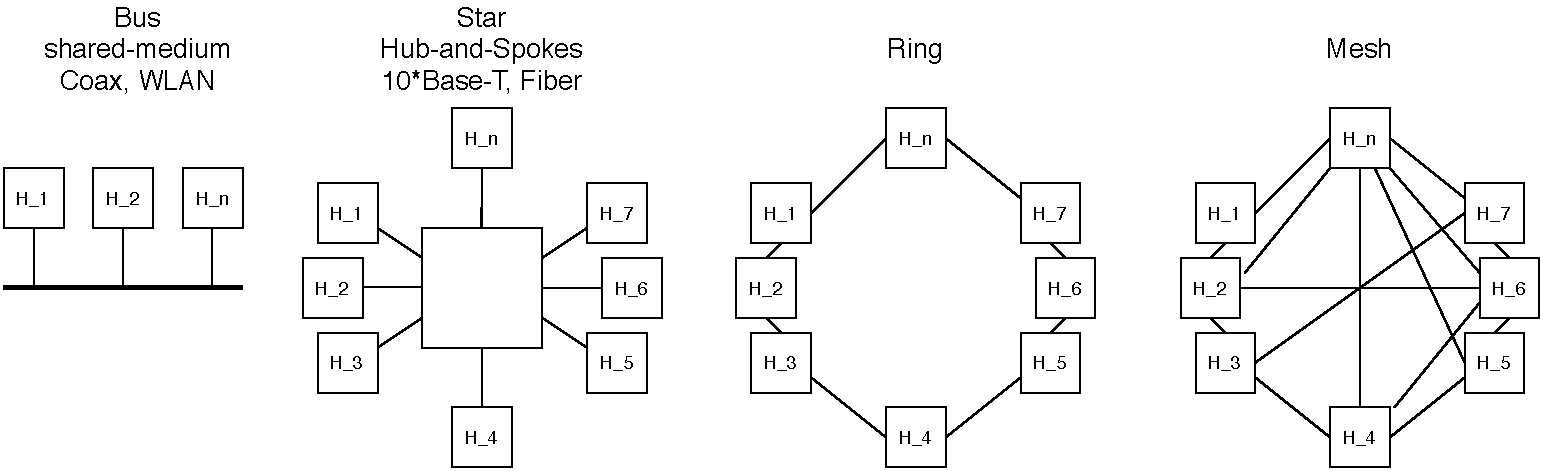
\includegraphics[width=11cm]{physical-architectures}

\begin{tiny}
Heute \"ublich:
\begin{itemize}
  \item ``im Kleinen''\footnote{Campus}: Sternf\"ormige Verkabelung, ``Bus''/WLAN
  \item ``im Grossen''\footnote{Internet, zwischen Provider}: Vermascht
  \item oft auch (hierarchische) Mischformen
\end{itemize}
\end{tiny}
\end{frame}


\begin{frame}
\frametitle{Layer-2: Fehlererkennung/-korrektur}
Jede physikalische \"Ubertragung ist St\"orungen unterworfen:

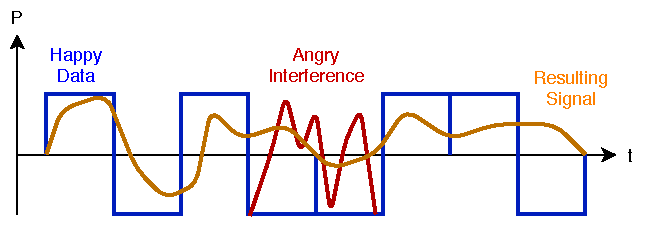
\includegraphics[height=2cm]{EM-error}

Das Zusammenfassen der einzelnen Bits in ``Frames'' bietet auch die M\"oglichkeit {\em Redundanz}\footnote{``mehr Daten ohne mehr Informationsinhalt''} zu diesen Einheiten zuzuf\"ugen. Dadurch wird eine Fehlererkennung und eventuell eine Fehlerkorrektur m\"oglich:
\end{frame}


\begin{frame}
\frametitle{Kommunikationstechniken Fehlererkennung/-Korrektur/-Vermeidung}
\begin{itemize}
  \item[ARQ]: ``automatic repeat reqeust'' -- eine Quittung (oder Timeout=``keine Quittung'') wird gesendet. In TCP/IP erst auf L4: TCP
  \item[FEC]: ``forward error correction'': es werden {\em redundante} Daten gesendet, der Empf�nger kann die Nachricht pr\"ufen und je nach Verfahren korrigieren\footnote{besonder f\"ur ``Broadcast''-Kommunikation n\"utzlich, wenn keine Quittung gesendet werden kann}. Im einfachsten Fall wird die Sendung $n>2$ mal wiederholt
  \item[Hybrid]: der Empf\"anger kann eine korruptes Frame neu anfordern\footnote{funktioniert z.B. bei Ethernet nicht, da die Adressierung auch im FEC eingeschlossen ist}
\end{itemize}
\end{frame}









\begin{frame}
\frametitle{Fehlererkennende Codes}
\small
F\"ur die Erkennung von \"Ubertragungsfehlern, werden verschiedene Methoden
eingesetzt, bei denen zus\"atzliche \alert{Redundanz} in die Daten eingef\"ugt wird. 
Fehlererkennung ist immer ein Tradeoff zwischen zus\"atzlicher Redundanz und Auftretenswahrscheinlichkeit des Fehlers.
\begin{description}
\item [Parit\"atsbit(s):] Pro Frame/Byte zus\"atzliche Bit(s), welche die Anzahl der ''1'' reflektieren\footnote{z.B. gerade Anzahl $\rightarrow$Parit\"atsbit=''0''} (odd/even).
\item [Pr\"ufsummen:] z.B. CRC, Cyclic Redundancy Check. Es werden nach bestimmten
        Regeln Checksummen \"uber die Daten gebildet und mitgesendet, auf der Empfangsseite 
        wird die Pr\"ufsumme erneut gebildet und mit der mitgesendeten verglichen.
\item [``Robuste Codes'':] Die ''Bit-Differenz'' der Codew\"orter wird ausgenutzt, damit
        Fehler erkannt und korrigiert werden k\"onnen. Ein 8-Bit Code mit nur 4 Code-Points: \\00000000, 00001111, 11110000, 11111111,\\
        Kann mit einem ''Abstand'' von mindestens 4 Bit definiert werden: 
        ({\bfseries Hammingdistanz}) damit werden bis zu $n-1$ Bit Fehler erkannt.
\end{description}
\begin{tiny}\[Folie: Degen\]\end{tiny}
\end{frame}




\begin{frame}
\frametitle{Beispiel f\"ur Parit\"atsbits}
\begin{center}
\begin{tiny}\[Folie: Degen\]\end{tiny}
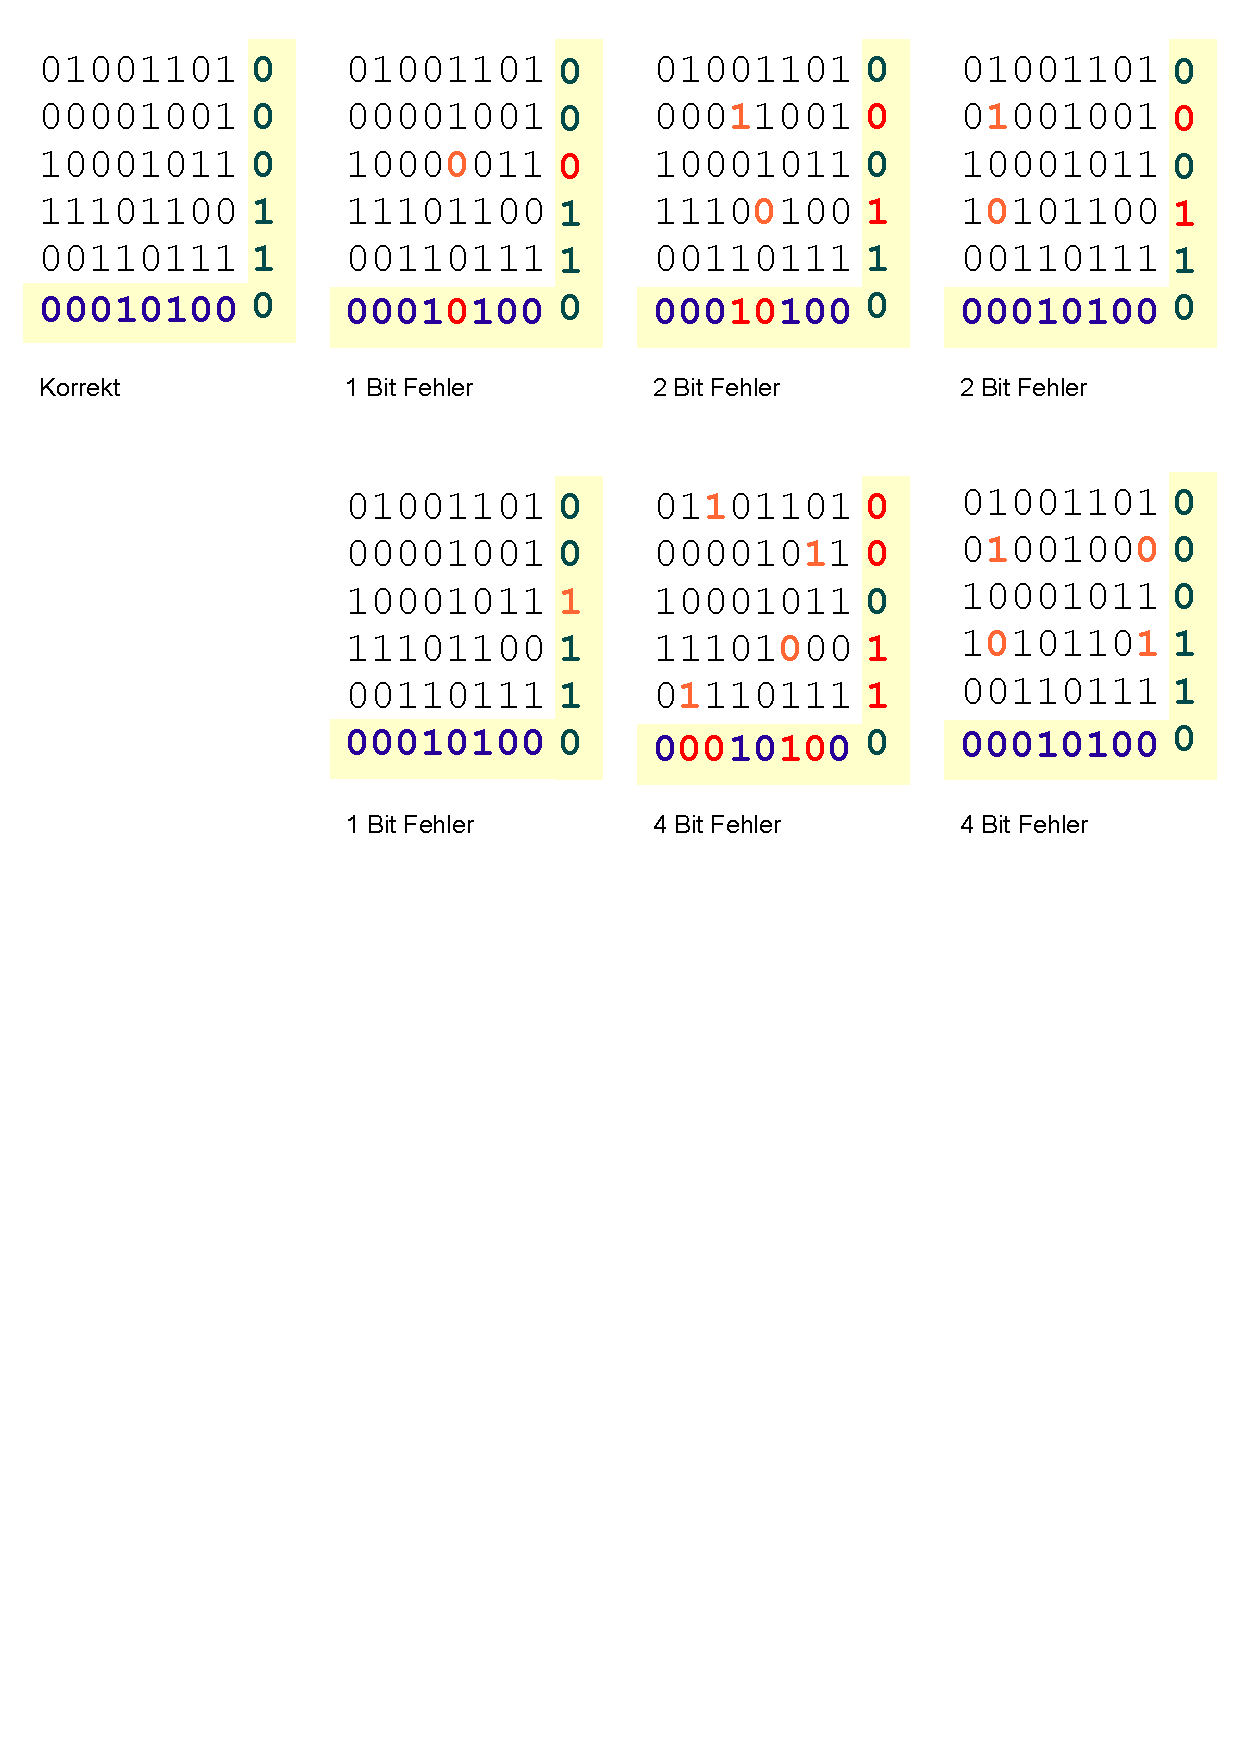
\includegraphics[width=0.8\textwidth]{blockparity.pdf}
\end{center}
\end{frame}






\begin{frame}
\frametitle{Hammingcodes}

Hamming-Codes erm\"oglichen ein gutes Redundanz-Verh\"altnis\footnote{...das mit steigender Bitzahl/Blockgr\"osse besser wird} -- d.h. m\"oglichst wenig redundante Daten. Dies wird erreicht mit einem ``Block''-Parit\"atsschema:

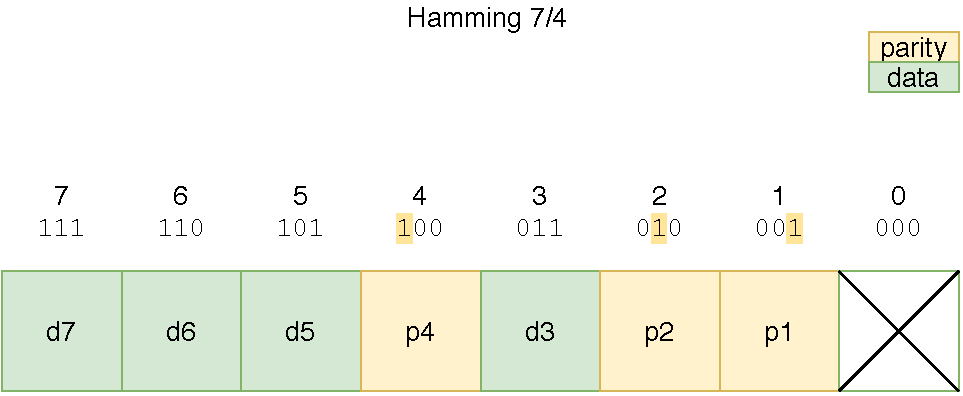
\includegraphics[height=2.5cm]{hammingcode}

$p_1 = d_3 \oplus d_5 \oplus d_7$

$p_3 = d_3 \oplus d_6 \oplus d_7$

$p_4 = d_5 \oplus d_6 \oplus d_7$

\myurl{https://en.wikipedia.org/wiki/Hamming_code}

\myurl{https://www.youtube.com/watch?v=b3NxrZOu_CE}

\myurl{https://www.youtube.com/watch?v=b3NxrZOu_CE}
\end{frame}






\begin{frame}
\frametitle{CRC -- Cyclic Redundancy Check}
CRC berechnet eine Pr\"ufsumme {\em fester L\"ange} f\"ur beliebig lange Nachrichten\footnote{``undetected error rate'' wird aber schlechter bei sehr grossen Verh\"altnissen. Ethernet 1500 Bytes -> 32 Bit CRC}.  Dazu wird ein {\em Generatorpolynom}�bin\"ar mit der Nachricht verarbeitet\footnote{die Nachricht wird ohne \"Ubertrag dividiert}, z.B:


\begin{tiny}
Generator = $x^3 + x + 1$ wird als Folge von 0 (kein Faktor) oder 1 (Faktor 1) codiert: 1011

\verbatiminput{crc-example.txt}
\end{tiny}

Beispiel von \myurl{https://en.wikipedia.org/wiki/Cyclic_redundancy_check} geklaut
\end{frame}









\begin{frame}
\frametitle{}
\end{frame}








\begin{frame}
\frametitle{Layer-2: Stack (Ethernet)}
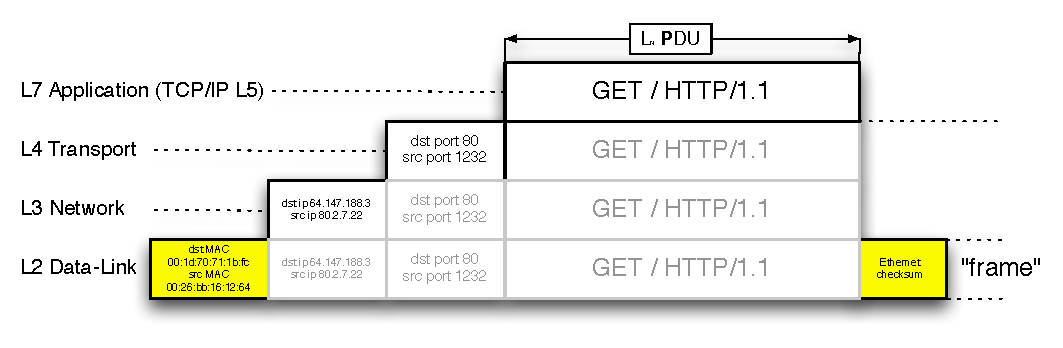
\includegraphics[width=12cm]{stack-pdu-sdu}
\end{frame}


\begin{frame}
\frametitle{L2 Responsibilities (Ethernet)}
\begin{itemize}
	\item {\em framing}/``packaging'' of data for transport over links (ie, between \emph{adjacent} nodes/LAN\footnote{Local Area Network: typical in-house network connected to the Internet via a Router. WAN/Wide Area Network consist of many LANs $\rightarrow$ Internet})
	\item implementation of device {\em addresses} in LAN\footnote{ie, ``local''}
	\item Ethernet/IEEE-802.3 allows for multicast- and broadcast destination\footnote{message to some or all nodes on LAN}
	\item {\em Error detection} using a 32-bit CRC\footnote{err'd frames are simply dropped by bridges, routers, hosts. Ponder about the reason for this\ldots}
	\item Ethernet L2 does {\em not} assure delivery\footnote{ie, the layers above must handle lost messages} (ie. no acknowledges sent, no attempt to retransmit)
\end{itemize}
\end{frame}

\begin{frame}
\frametitle{L2 Factlets}
\begin{itemize}
	\item{messages on a Ethernet LAN are called {\em frames}}
	\item most abundant LANs/L2-Networks today are 802.3/Ethernet and 802.11/Wireless
	\item devices for {\em building} LANs: L1:Hub/Repeater and L2:Bridge/Switch
	\item devices {\em interconnecting} LANs to other LANs or the ``outside world'': L3:Router or L3+:Firewall/Router
	\item L2 addressing is of {\em local} \footnote{there is no need for your computer to know the L2 address of a webserver in the Internet} interest only!
	\item{a Link/L1 forms a ``collision domain'', transmissions from different devices may ``collide'' on a single wire/Hub} 
	\item{a LAN/L2 denotes a ``broadcast domain'': \texttt{0xFF:FF:FF:FF:FF:FF} destination is sent to all nodes on the LAN\footnote{it is {\em limited}, ie it never leaves the LAN via a router}}
	\item{802.x/Ethernet is a TDM\footnote{Time Domain Multiplexing} network}
\end{itemize}
\end{frame}


\begin{frame}
\frametitle{L2 Frame-Header/Metadata}
encapsulates -- ``frames'' -- a certain\footnote{on Ethernet maximum 1518 Bytes - layer-2 metadata, minimum 64 Bytes} amount of data\footnote{the ``payload'' from Layer-3, this is the ``SDU'' service-data-unit on Layer-2} from above layer with metadata:
\begin{itemize}
	\item \textbf{Preamble}: a special synchronize sequence\footnote{\myurl{http://en.wikipedia.org/wiki/Ethernet\_frame}}
	\item \textbf{Address}: destination- and source-address of adjacent nodes
	\item \textbf{Type}: identifies encapsulated data (type of SDU/upper-layer), eg \texttt{0x0800} for IP
	\item \textbf{Frame Checksum}\footnote{CRC32}: allows the destination node to check consistency of data received
\end{itemize}
\end{frame}

\begin{frame}
\frametitle{L2 Addressing (1/2)}
\begin{itemize}
	\item{Ethernet L2/MAC addresses consists of 6 Bytes (3 vendor-id\footnote{\myurl{https://db.uga.edu/network/public/vendorcode.cgi}}, 3 serial)}
	\item{this allows for (theoretical) $2^{48}\sim 256$ trillion addresses}
	\item{the usual notation for MAC addresses are hex\footnote{sometimes identified by \texttt{0x}-prefix} bytes seperated by ``:''}
	\item{MAC adresses are guaranteed\footnote{theoretically\ldots most OS/network cards allows you to alter this address and sometimes the vendor just blows it} to be unique}
	\item{\texttt{0xFF:FF:FF:FF:FF:FF} is the {\em broadcast} \footnote{``to all'', limited to the LAN of course} destination address}
	\item{any address with the \texttt{0x\_1:\_\_:\_\_:\_\_:\_\_:\_\_} bit set is {\em multicast} \footnote{eg. to ``all routers'' in LAN}}
\end{itemize}
\end{frame}

\begin{frame}
\frametitle{L2 Addressing (2/2)}

\begin{itemize}
\item MAC/L2-Addresses exhibit no ``grouping'' network-coherence/pattern \begin{tiny}\verbatiminput{arp-table.txt}\end{tiny}
\item the address is specific to the device and not the location\footnote{ie, the address stays the same: on campus or at home}
\end{itemize}
\begin{block}{}
MAC-addresses are LAN/{\em local}-only
\end{block}
\end{frame}



\begin{frame}
\frametitle{L2 Interlude}
\begin{itemize}
	\item{find your computers MAC address\footnote{UNIX: \texttt{ifconfig}, Microsoft Windows: \texttt{ipconfig /all}}}
	\item{find the vendor of your computers NIC\footnote{Network Interface Card}}
	\item{find other MACs your computer had conversation with\footnote{\texttt{arp -a}, add another \texttt{-n} on UNIX for faster responses}}
	\item{find the vendor of the router\footnote{``default gateway''} connecting you to the internet\footnote{this is actually a L3 theme\ldots use \texttt{netstat -rn} to find the routers IP and locate the corresponding MAC in the \texttt{arp -a} output}}
	\item{find the MAC of your neighbours PC\footnote{use \texttt{ping {\em IP}} first then issue \texttt{arp -a} once again}}
	\item{find the MAC of \texttt{www.eff.org}}
	\item{listen to the network chit-chat using \texttt{tcpdump} (on \texttt{netbox}). Try to identify L2-broadcast, multicast and unicast}
\end{itemize}
\end{frame}

\begin{frame}
\frametitle{L2 Bridging 1/2}
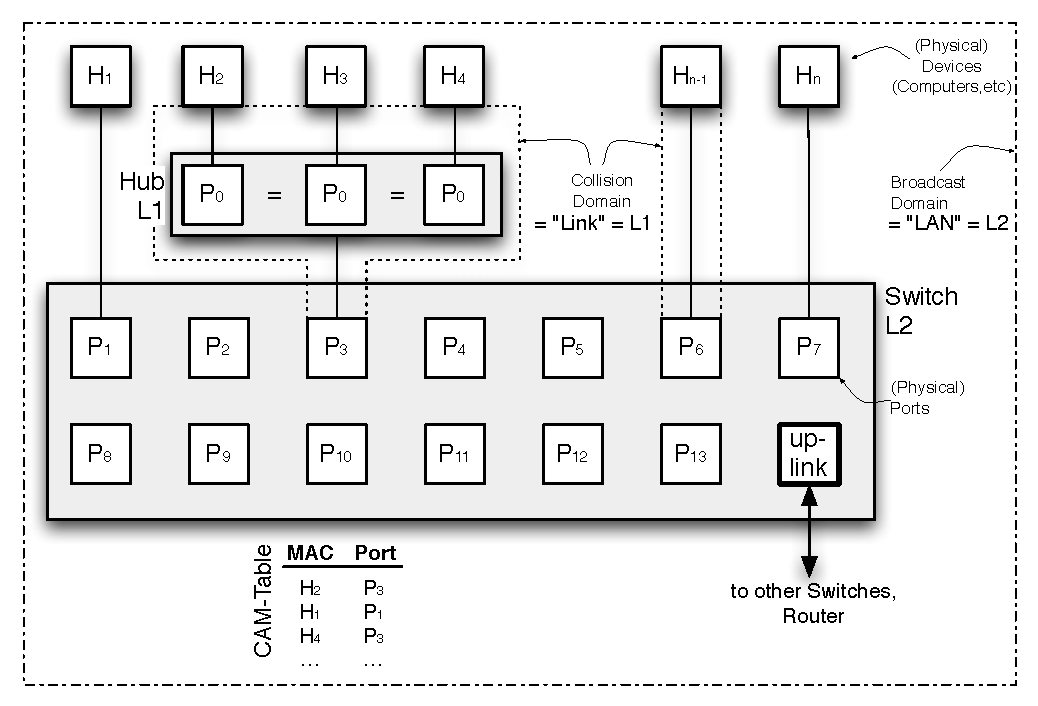
\includegraphics[width=12cm]{bridge}
\end{frame}

\begin{frame}
\frametitle{L2 Bridging 2/2}
\begin{itemize}
	\item{{\em bridges} are devices to extend the reach of a LAN. The resulting network is still a single LAN}
	\item{multiport\footnote{anything with more than a few ports} bridges are called (L3) {\em switches}}
	\item{bridges analyze the destination address of a frame and transmit it only on specific port(s)}
	\begin{itemize}
	\item{\ldots thus providing some ``privacy''\footnote{try yourself: use \texttt{wireshark} or \texttt{tcpdump} and see if you can spy on your neighbous traffic}}
	\item{this is achieved by building a MAC-address/port lookup table by storing the {\em source} MAC-address along with the receiving port number}
	\end{itemize}
	\item{as long as a particular destination MAC-address is not known, frames must be {\em flooded} out to all except the receiving port}
	\item{broadcast frames are send out on all ports except on the receiving one}
\end{itemize}
\end{frame}

% Alix
%eth0      Link encap:Ethernet  HWaddr 00:0d:b9:1a:01:3c  
%          inet addr:192.168.1.46  Bcast:192.168.1.255  Mask:255.255.255.0
%          inet6 addr: fe80::20d:b9ff:fe1a:13c/64 Scope:Link
%          UP BROADCAST RUNNING MULTICAST  MTU:1500  Metric:1
%          RX packets:63769 errors:0 dropped:0 overruns:0 frame:0
%          TX packets:7151 errors:0 dropped:0 overruns:0 carrier:0
%          collisions:0 txqueuelen:1000 
%          RX bytes:16734971 (15.9 MiB)  TX bytes:999474 (976.0 KiB)
%          Interrupt:10 Base address:0x2000 
%
%eth1      Link encap:Ethernet  HWaddr 00:0d:b9:1a:01:3d  
%          BROADCAST MULTICAST  MTU:1500  Metric:1
%          RX packets:0 errors:0 dropped:0 overruns:0 frame:0
%          TX packets:0 errors:0 dropped:0 overruns:0 carrier:0
%          collisions:0 txqueuelen:1000 
%          RX bytes:0 (0.0 B)  TX bytes:0 (0.0 B)
%          Interrupt:15 Base address:0x8000 


% collisions and collision-domain
\begin{frame}
\frametitle{L2 CSMA/CD, Collision-Domain}
\begin{itemize}
  \item{CSMA: Carrier Sense Multiple Access/Collision Detection}
	\item{since the cable/medium\footnote{in case of twisted-pair cables the send/receive lines are physically seperated allowing for full-duplex traffic. Traditional coax-cables are half-duplex only} allows for at a single transmission only at any given time (TDM), the sender constantly monitors its transmission and cancels it in case of noise: {\em collision detection}}
	\item{such a L1-segment\footnote{single broadcast-medium cable (coax) or repeater/hub interconnected} is called a ``collision-domain''}
	\item{bridged seperates ``collision-domains'', thus a end-device connected to a switch has its private collision-domain\footnote{and will never encounter collisions at all if configured correctly}}
	\item {\bfseries today there are no longer collisions on wired networks}\footnote{assuming all cabling is centralized in switches},\\ in WLAN CSMA still applies, though
\end{itemize}
\end{frame}


% cut-through vs store-and-forward
\begin{frame}
\frametitle{L2 Bridging: Cut-Through vs Store-and-Forward}
\begin{itemize}
	\item{traditionally bridges/switches receives a whole frame and forwards it if the frame-checksum matches}
	\item{this adds a certain {\em latency} \footnote{a delay, in this case dependent of the frame-length} to the transmission}
	\item{some bridges/switches offer a {\em cut-through} forwarding mode, where the frame is forwarded as soon as the destination-address is received}
	\item{this mode allows for a {\em constant} and minimal latency}
	\item{in case of line-noise, the bridge may forward defective frames in cut-through mode}
	\item{advanced bridges mitigate this problem by fall-back to store-and-forward mode in presence of errors}
\end{itemize}
\end{frame}


% Loops, Spanning-Tree
\begin{frame}
\frametitle{L2 Briding: Loops and avoidance of}
\begin{itemize}
	\item{complex LANs with multiple bridges may form {\em loops} \footnote{try this at home: ``short-circuit'' your (auto-crossover) switch by connecting a cable back-to-back}}
	\item{especially broadcast frames may lead to a (broadcast) {\em storm}}
	\item{advanced bridges employ a {\em spanning-tree \footnote{IEE 802.3D STP Spanning Tree Protocol: an application of the Djikstra-Algorithm, we'll study this in L3 OSPF}} protocol to avoid this}
\end{itemize}
\end{frame}


% VLAN
\begin{frame}
\frametitle{L2 Bridging: VLAN}
\begin{itemize}
	\item{advanced bridges allow for {\em Virtual LANs} (VLANs)}
	\item{VLANs are seperated LAN/L2-segments\footnote{ie, a router is required to interconnect VLANs}}
	\item{the L2 metadata is extended by a VLAN-identification number}
	\item{a physical port on the bridge can be configured to allow for one VLAN only\footnote{the VLAN-id is {\em stripped}�from the metadata} -- usually to connect to end-devices}
	\item{physical ports may also be configured to operate in {\em trunking} mode -- usually in bridge-to-bridge {\em aggregated} link or to allow for advanced end-devices to seperate VLANs internally}
	\item{typical applications: seperate external-, internal- and server-LAN for security reasons\footnote{this is considered bad practice}}
\end{itemize}
\end{frame}

\begin{frame}
\frametitle{L2: References for ND03}
\begin{itemize}
\item \myurl{http://en.wikipedia.org/wiki/Ethernet\_frame}, \myurl{http://en.wikipedia.org/wiki/Ethernet\_II\_framing}
\item \myurl{http://en.wikipedia.org/wiki/802.3}
\item \myurl{http://en.wikipedia.org/wiki/IEEE_802.1D}
\item \myurl{http://en.wikipedia.org/wiki/Bridging\_(networking)} especially the part ``bridging makes no assumptions about where in the network a particular address is located'' $\rightarrow$ ``flooding''
\item \myurl{http://en.wikipedia.org/wiki/Frame\_(networking)}
\item \myurl{https://db.uga.edu/network/public/vendorcode.cgi}, MAC vendor
\end{itemize}
\end{frame}

%\begin{frame}
%\frametitle{Layer-3}
%\begin{itemize}
%	\item{packet-switched network, best-effort (ie, no assured delivery/acknowledge/resend on L3)}
%	\item{arp, determine MAC of peer or router}
%	\item{end-to-end addressing}
%	\item{reachability on L3: \texttt{ping}, \texttt{traceroute}/\texttt{tracert}}
%	\item{address-format, classes}
%	\item{subnets, CIDR}
%	\item{routing-table, forwarding, routing-protocol manages routing-table}
%	\item{routing-protocols}
%\end{itemize}
%\end{frame}


\end{document}
